\section{Incremental Deployment} \label{sec:incremental} 

Section~\ref{sec:base} covered the full design that places zero-trust in the CT
landscape by challenging the logs to prove certificate inclusion with regards to
trusted STHs in the Tor consensus.  If no such proof can be provided, the
suspected evidence of log misbehavior is reported to a trusted CT auditor that
follows-up on the incident, which involves human intervention if an issue
persists.  The proposed design modifies the Tor consensus, Tor relays, and Tor
Browser.  It also requires development and operation of a trusted auditor
infrastructure.  The current lack of the latter makes it unlikely that we will
see adoption of CTor in its full potential anytime soon, and begs the question
of increments that help us get there in the future. Therefore, we additionally
propose two incremental designs in this section.

\begin{figure*}
    \centering
	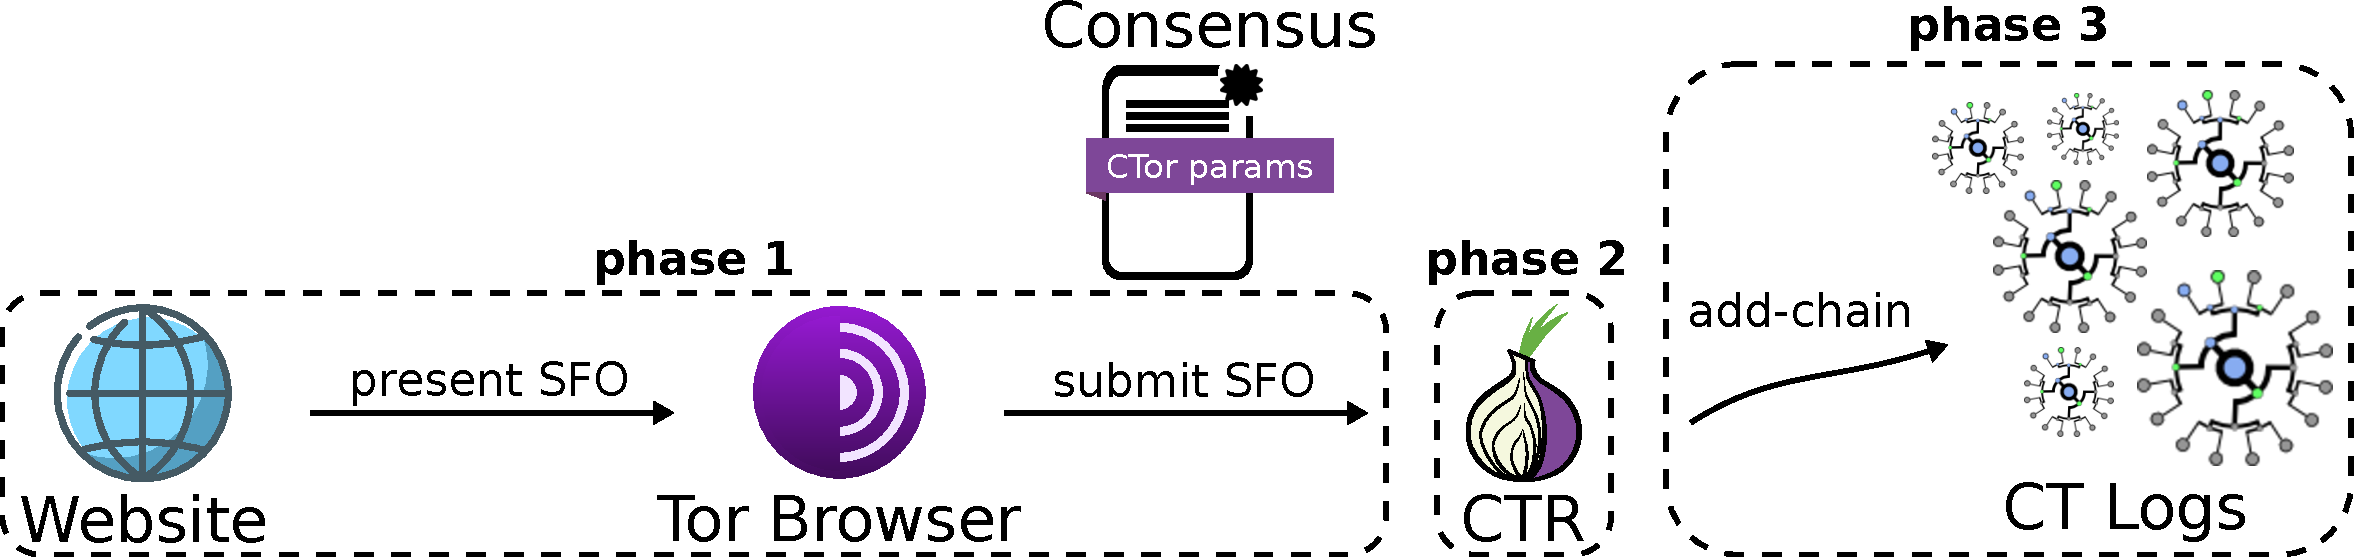
\includegraphics[width=0.8\textwidth]{img/design-incremental}
	\vspace{-8px}
	\caption{%
		Incremental design that can be deployed without any
		trusted CT auditors.  Tor Browser still submits SFOs to CTRs on
		independent Tor circuits for the sake of privacy and security.  After
		CTR buffering, the submitted certificates are \emph{cross-logged} by
		adding them to independent CT logs (selected at random) that the
		attacker does not control (inferred from accompanied SCTs).
	}
	\label{fig:cross-log}
	\vspace{-10px}
\end{figure*}

Without the ability to rely on CT auditors, trust needs to be shifted elsewhere
because we cannot expect relay operators to take on the role.  At the same time,
an incremental proposal needs to improve upon the status quo of
pairwise-independently trusted CT logs. These observations lead us towards the
trust assumption that \emph{at least some} of the CT logs are trustworthy. Such
an assumption is suboptimal, but it does provide a real-world security
improvement by significantly raising the bar from weakest-link(s) to quite the
opposite.

The smallest change of the full design would be for watchdogs to report
suspected certificate mis-issuance to all CT logs, simply by using the public
\texttt{add-chain} API to make the SFO's certificate chain transparent.  This
has the benefit of holding the CA accountable if \emph{some} log operator is
benign.  Given that our attacker is risk-averse, reporting to a single
independent log\footnote{The independent log need not be trusted by the browser,
i.e., it could be specified separately in the Tor consensus.  An operator that
runs such a log would help distribute trust and facilitate auditing.
Appendix~\ref{app:ct-trust-anchors} provides details on today's log ecosystem.}
that issued none of the accompanied SCTs would likely be sufficient.  There is
also room for further simplification: there is no point in challenging the logs
to prove inclusion if the fallback behavior of no response only makes the issued
certificate public, not the associated SCTs. Thus, CTRs could opt to cross-log
immediately \emph{without ever distinguishing between certificates that are
benign and possibly fraudulent}.  This results in the incremental design shown
in Figure~\ref{fig:cross-log}, which initially removes several system
complexities such as extra-info metrics, auditor infrastructure, watchdog
collaborations, and inclusion proof fetching against trusted STHs in Tor's
consensus.

The drawback of certificate cross-logging is that the misbehaving CT logs cannot
be exposed.  There is also a discrepancy between cross-logging and encouraging
the CT landscape to deploy reliable CT auditors.  We therefore suggest a
minimal change to the basic cross-logging design that addresses both of these
concerns.  This change is unfortunately to the API of CT logs and not Tor.  The
proposed change is to allow cross-logging of a certificate's issued SCTs, e.g.,
in the form of an \texttt{add-sfo} API that would replace \texttt{add-chain}
in Figure~\ref{fig:cross-log}.
This means that CTRs could expose both the mis-issued certificate and the logs
that violated their promises of public logging.  At the same time, the
infrastructural part of a CT auditor is built directly into existing
CT logs:
	accepting SFOs that need further investigation.
Such an API would be an ecosystem improvement in itself, providing a
well-defined place to report suspected log misbehavior on-the-fly
\emph{casually}, i.e., without first trying to resolve an SFO for an extended
time period from many different vantage points and then ultimately reporting it
manually on the CT policy mailing list.

\textbf{Security sketch.} 
There are no changes to phase~1 because cross-logging is instantiated at CTRs.
Phases~3--4 are now merged, such that the encountered certificates are added to
independent CT logs that the attacker does/may not control.  Watchdogs are no
longer needed since either the certificates are added to a log that the attacker
controls, or they are not (which makes them public).  The other main difference takes place in phase~2,
during which CTRs buffer SFOs.  The buffer time used to be lengthy due to taking
early signals and MMDs into account, but it is now irrelevant as no inclusion
proofs are fetched.  The expected buffer time can therefore be shortened down
to \emph{minutes} that follow only from the randomness in the
\texttt{audit\_after} timestamp (for the sake of privacy), making network-wide
flushes impractical while at the same time reducing the time that a mis-issued
certificate stays unnoticed:
	a benign log is likely to add an entry before all MMDs elapsed.

The extended cross-logging also aims to expose log misbehavior.  As such, it is
paramount that no cross-logged SFO becomes public before the issuing CT logs can
merge the mis-issued certificate reactively to avoid catastrophic impact. This
could be assured by buffering newly issued SFOs longer as in the full design,
which brings back the threat and complexity of minor impact scenarios. Another
option that is appealing for Tor (but less so for CT) is to operate the
\texttt{add-sfo} API with the expectation of \emph{delayed merges} that account
for MMDs before making an SFO public, effectively moving lengthy buffering from
CTRs to CT logs with persistent storage.  Trillian-based CT logs already support
delayed merges of (pre)certificates, see
\texttt{sequencer\_guard\_window}~\cite{delayed-merge}.
